% !TEX program = xelatex
\documentclass[10pt,twocolumn,letterpaper]{article}
\usepackage[margin=0.72in,columnsep=0.24in]{geometry}
\usepackage[T1]{fontenc}
\usepackage{mathptmx}
\usepackage{amsmath,amssymb,bm}
\usepackage{graphicx,booktabs,array,microtype}
\usepackage[font=small,labelfont=bf]{caption}
\usepackage[numbers,sort&compress]{natbib}
\usepackage{xcolor}
\usepackage[breaklinks,colorlinks,allcolors=blue!45!black]{hyperref}
\usepackage{url}
\usepackage{xurl,titlesec,float}
\usepackage{placeins}
\titleformat{\section}{\large\bfseries}{\thesection}{0.7em}{}
\titleformat{\subsection}{\normalsize\bfseries}{\thesubsection}{0.7em}{}
\titlespacing*{\section}{0pt}{1.8ex plus .4ex minus .2ex}{.75ex plus .2ex}
\titlespacing*{\subsection}{0pt}{1.5ex plus .3ex minus .2ex}{.6ex plus .2ex}
\urlstyle{same}
\raggedbottom
\setlength{\emergencystretch}{1.5em}
\setlength{\parskip}{0pt}
\newcommand{\dex}{\,\mathrm{dex}}
\newcommand{\clip}{\operatorname{clip}}
\newcommand{\RMSE}{\operatorname{RMSE}}
\newcommand{\MAE}{\operatorname{MAE}}
\newcommand{\E}{\mathbb{E}}
\newcommand{\R}{\mathbb{R}}
\newcommand{\code}[1]{\texttt{\small #1}}
\title{Physics-Constrained Reinforcement Learning for Graph Sparsification in Cosmological Graph Neural Networks:\\A Controlled Empirical Study}
\author{Cosmic-Net project\\\small Supervisor-review draft; author list and affiliations to be confirmed}
\date{16 October 2026}
\begin{document}
\maketitle
\begin{abstract}
Learned graph sparsification may reduce the interactions processed by cosmological graph neural networks, but fewer edges do not by themselves imply faster or more accurate inference. We examine Cosmic-Net, an edge-conditioned halo-mass predictor with a reinforcement-learning selector, using a completed four-notebook experimental campaign. A physical-pair representation separates reciprocal edge copies from self-loops, and a shared feasibility-aware decoder enforces exact pair budgets and excludes physical isolates. On 82 held-out halo graphs from one legacy TNG100-labelled catalog, nominal 40\% retention realizes 40.30\% mean pair retention. The full graph achieves an RMSE of $0.114797\dex$, compared with $0.136160\dex$ for reinforcement learning and $0.136900\dex$ for gradient~$\times$~input selection. The observed 0.54\% advantage over that control is inconclusive: the paired RMSE difference is $-0.000739\dex$, with a 95\% bootstrap interval of $[-0.014508,+0.013582]\dex$ and permutation $p=0.9192$. Reinforcement learning is 18.61\% worse than the full graph and approximately $56\times$ slower in the measured inference region. At a separate 50\% budget, label-free test-time adaptation improves aggregate RMSE by 0.558\% while increasing latency $2.50\times$; paired predictions are unavailable. Unresolved historical target semantics, incomplete backbone provenance, and absent seed and volume replications restrict interpretation. The study establishes a traceable constrained benchmark and documents failure modes; it establishes neither an accuracy nor an efficiency advantage.
\end{abstract}
\noindent\textbf{Keywords:} graph sparsification; halo mass inference; reinforcement learning; physical constraints; empirical evaluation

\section{Introduction}
Dark matter halo masses connect galaxy populations to their gravitational environments. A galaxy system provides a variable number of tracers with correlated positions, velocities, and intrinsic properties. Graph neural networks (GNNs) offer a natural representation of these data: galaxies become nodes, relationships become edges, and permutation-invariant pooling produces a halo-level estimate. Existing work already demonstrates GNN halo-mass inference across simulation suites \citep{villanueva2022,garuda2024}. The question here is narrower: how much predictive information survives when interactions in an existing predictor are removed under explicit structural constraints?

Sparsification has several possible purposes, including reducing computation, identifying predictive relationships, or limiting communication. These purposes require different evidence. Preserving predictions does not establish a physical explanation, and removing edges does not establish a speedup when a selector itself requires a full model pass. A scientific evaluation must therefore measure accuracy, selection feasibility, and total inference cost together, against competitive selectors with identical final budgets.

Cosmic-Net combines an edge-conditioned GNN with a learned pair selector and a relative virial-inspired reward. We report its completed A--D campaign as a controlled empirical study of that implemented system. The campaign provides a useful test bed for exact budget accounting and constrained evaluation, despite unresolved provenance in its historical catalog and frozen checkpoint. We retain the explicit research label \code{legacy\_total\_radius}; the measurements are conditional results on that artifact, rather than a certified measurement of a particular spherical-overdensity mass definition.

The study has three aims. First, we describe the actual selection and reward implementation, including the difference between repaired training actions and exact-budget inference. Second, we compare seven selectors using the same frozen predictor, halo population, and physical-pair decoder. Third, we quantify uncertainty in small observed differences and account for selection overhead. The main result is a qualified negative one: at 40\% nominal retention the learned policy is less accurate than the full graph, its point advantage over gradient~$\times$~input is unresolved, and the implemented inference path is substantially slower. These observations motivate concrete changes in evaluation and deployment design without asserting that learned sparsification cannot be useful elsewhere.

\section{Related Work}
\paragraph{Cosmological graph learning.}
\citet{villanueva2022} infer halo masses from member-galaxy properties using GNNs trained on CAMELS simulations. \citet{garuda2024} study cluster halo-mass prediction with spatial and kinematic graph information in IllustrisTNG. These establish the broader task and motivate representing galaxy systems relationally. Their reported errors cannot be ranked against this study's errors because data selection, target definitions, feature availability, and validation domains differ. CAMELS varies cosmology and astrophysical prescriptions \citep{camels2021}; this campaign does not implement that form of independent-domain evaluation.

\paragraph{Learned graph sparsification.}
NeuralSparse learns to remove task-irrelevant edges under downstream supervision \citep{zheng2020}. SparRL uses reinforcement learning for graph reduction with user-defined objectives \citep{wickman2021}. Thus neither neural edge selection nor RL sparsification is new in itself. Cosmic-Net's combination of a halo predictor, physical-pair budgets, feasibility checks, and a stellar-dynamical proxy is the object of this evaluation. We do not claim a new general sparsification algorithm or a reproduced comparison with those published systems. The implemented learned baseline is a raw-feature saliency-distilled selector, not NeuralSparse or PGExplainer.

\paragraph{Message passing and reliable evaluation.}
The backbone uses edge-conditioned convolutions \citep{simonovsky2017}. The selector uses score-function policy gradients \citep{williams1992}, with ordered sampling without replacement. Monte Carlo dropout supplies the adaptation uncertainty proxy \citep{gal2016}; its theoretical motivation alone does not certify calibration in this application. The need to report uncertainty beyond a single RL score is well established \citep{agarwal2021}. Our paired halo-level analysis addresses conditional test-sample uncertainty, but cannot substitute for independent training runs or simulation volumes. Bootstrap intervals \citep{efron1987} and multiplicity adjustment \citep{holm1979} are used to make that distinction visible.

\section{Scientific Background}
The dynamical motivation is the approximate virial relation $2T+W\simeq0$ for an equilibrated bound system. A graph over galaxies, however, contains tracers rather than the full gravitating matter distribution. Stellar masses, subhalo velocity dispersions, and pair separations do not directly determine the halo's total kinetic and potential energy. We consequently interpret the implemented physics term as a regularizer preserving a graph-dependent proxy, not as a conservation law or an equilibrium certificate.

The prediction target is the stored logarithmic mass,
\begin{equation}
 y_g=\log_{10}(M_{g,\mathrm{stored}}/M_\odot),\qquad
 \hat y_g=f_\theta(G_g).
\end{equation}
Errors in this logarithm are reported in dex. Although the loader's API path names \code{Group\_M\_Crit200}, the legacy CSV contract explicitly records an unknown historical target definition. We therefore do not relabel the campaign target as independently verified $M_{200\mathrm{c}}$. The intended task is halo-mass inference; the measured task is regression against these specific historical labels.

\section{Dataset and Graph Construction}
\label{sec:data}
The campaign reads a TNG100-labelled, snapshot-99 ($z=0$) clustered CSV. IllustrisTNG provides the simulation context \citep{nelson2017}; that citation does not certify this derived catalog's acquisition history. The supplied file has 5,378 rows and produces 541 halo graphs, divided into 378 training, 81 validation, and 82 test graphs with seed 42 and nominal 70/15/15\% proportions. The split is at halo level within one volume. Identical file and model hashes and split identities are recorded across the campaign. They establish artifact identity, not the absence of leakage during the backbone's earlier training.

For a halo let $V=\{1,\ldots,N\}$ and let $D$ be the stored directed edge columns, including self-loops $L$. Non-self reciprocal copies are grouped into unordered physical pairs $U$; write $P=|U|$. The graph is $G=(V,D,X,A)$ with $X\in\R^{N\times4}$ and $A\in\R^{|D|\times5}$. Each node carries
\begin{equation}
 x_i=\bigl(\log_{10}m_{*,i},\log_{10}\sigma_i,
             \log_{10}R_i,\log_{10}Z_i\bigr),
\end{equation}
using numerical values in $M_\odot$, km\,s$^{-1}$, Mpc, and dimensionless metallicity. The feature routine floors inputs at $10^{-10}$ before taking logarithms; ingestion also applies field-specific floors. In this CSV, $R_i$ represents total-subhalo half-mass radius, despite older comments describing a stellar radius. The exact historical metallicity acquisition also merits certification.

For $\Delta\bm r_{ij}=\bm r_j-\bm r_i$ and $\Delta\bm v_{ij}=\bm v_j-\bm v_i$, the edge vector is
\begin{equation}
\begin{split}
 a_{ij}=\bigl(&r_{ij},\|\Delta\bm v_{ij}\|_2,c_{ij},\ell_{ij},r^\perp_{ij}\bigr),\\
 c_{ij}&=\clip\!\left(\frac{\Delta\bm r_{ij}\cdot\Delta\bm v_{ij}}
 {r_{ij}\|\Delta\bm v_{ij}\|_2+10^{-8}},-1,1\right),\\
 \ell_{ij}&=x_{i,1}-x_{j,1},\quad
 r^\perp_{ij}=\|\Delta\bm r_{ij,xy}\|_2.
\end{split}
\end{equation}
Here $r_{ij}=\|\Delta\bm r_{ij}\|_2$. The signed mass-ratio feature reverses sign on exchanging endpoints; the other four attributes do not. The projected separation is an auxiliary feature alongside intrinsic three-dimensional information, not a complete observational feature contract.

The configured graph includes reciprocal pairs within 2.0 Mpc, self-loops, and a nearest-neighbor fallback for physical isolates, with symmetric coalescing. Geometry uses direct Euclidean differences, without a periodic minimum-image correction in this path. Historical CSV positions and radii are explicitly interpreted as ckpc/$h$ and converted to Mpc using $h=0.6774$; stellar masses are interpreted as logarithmic and halo masses as linear $M_\odot$. These are declared legacy conventions, not magnitude-based unit inference. The repository fetch script caps satellites at ten. The observed test graphs contain 15--45 physical pairs (median 45), so this campaign does not test large-graph scaling or complete rich-cluster membership.

\section{Full-Graph GNN Architecture}
\label{sec:gnn}
The configured backbone projects four node features to width 64, applies three edge-conditioned \code{NNConv} blocks of width 64, pools by the node mean, and predicts one scalar through a $64\to64\to32\to1$ head. Each edge MLP is $5\to64\to64\to4096$, producing a $64\times64$ message matrix. With column-vector notation, a block can be written as
\begin{align}
 u_i^{(l)}&=W_{\mathrm{root}}^{(l)}h_i^{(l)}+b^{(l)}
 +\frac{1}{|\mathcal N_D(i)|}\sum_{j\in\mathcal N_D(i)}
 W^{(l)}(a_{ji})h_j^{(l)},\\
 h_i^{(l+1)}&=h_i^{(l)}+operatorname{Drop}_{.05}
 \left[\phi\!\left(\operatorname{LN}(u_i^{(l)})\right)\right],
\end{align}
where $h_i^{(0)}=\operatorname{Drop}_{.05}[\phi(W_{\mathrm{in}}x_i+b_{\mathrm{in}})]$, $\phi$ is leaky ReLU with slope 0.1, and $\mathcal N_D(i)$ includes the stored self-loop. The root transform is additional to that loop. Pooling gives $c=N^{-1}\sum_i h_i^{(3)}$ and $\hat y=\operatorname{MLP}_{\mathrm{head}}(c)$, with dropout and activation between head linear layers. Dropout is disabled for deterministic prediction and enabled for the uncertainty draws.

The policy consumes the full-graph pre-pooling embeddings $h_i^{(3)}$ and their mean $c$. The primary comparison freezes $\theta$ throughout selection. Although the repository includes a supervised MSE plus virial-proxy backbone training path, its current configuration is not a complete training record for the historical checkpoint. We describe the represented forward architecture and verified frozen state; we do not assert that today's training defaults reconstruct its original optimizer, augmentation, or split history. Optional later backbone fine-tuning is reported separately.

\section{Physics-Constrained RL Sparsification}
\label{sec:method}
\subsection{Policy formulation and action space}
The decision is a one-step graph-level selection problem, rather than a multi-step control trajectory. The state consists of the graph's edge attributes, frozen node embeddings, and mean context. The policy does not receive the mass label. For a directed column $(i,j)$ it computes
\begin{equation}
 z_{ij}=\operatorname{MLP}_{\psi}
 \bigl[\phi(B_h\tilde h_i),\phi(B_h\tilde h_j),
       \phi(B_a\tilde a_{ij}),\phi(B_h\tilde c)\bigr].
\end{equation}
Affine maps include biases; their outputs have width 64, and the concatenated width-256 vector passes through $256\to64\to64\to1$ layers with leaky ReLU between them. Tildes denote train-fitted featurewise standardization, with scale floored at $10^{-4}$ and standardized values clipped to $[-10,10]$. One shared map $B_h$ projects endpoints and context. A physical-pair score $s_p$ averages logits over all stored non-self copies of pair $p$. Loops are excluded from stochastic actions.

At training epoch $e$ the requested keep fraction is
\begin{equation}
 q_e=0.9-0.5\min(1,e/40),\qquad k_e=\lceil q_eP\rceil.
\end{equation}
The action $o=(p_1,\ldots,p_{k_e})$ is an ordered sample of distinct pairs under a Plackett--Luce law,
\begin{equation}
 \pi_\psi(o\mid G)=\prod_{t=1}^{k_e}
 \frac{\exp s_{p_t}}{\sum_{p\notin\{p_1,\ldots,p_{t-1}\}}\exp s_p}.
 \label{eq:pl}
\end{equation}
The implementation sums the conditional log probabilities exactly. Training then adds pairs to cover physical isolates using independent pair priorities, expands membership to every reciprocal copy, and preserves loops. This repair can exceed $k_e$. The likelihood in Eq.~\ref{eq:pl} is the ordered action likelihood, not the likelihood of the repaired mask. Reward is evaluated on the repaired graph; the additive repair is part of the environment. This distinction prevents an incorrect claim that the historical policy was trained by exact constrained-mask likelihood optimization.

\subsection{Reward design}
\label{sec:reward}
For one graph, let $D'_0$ be retained non-self directed columns. Full and retained degrees $d_i,d'_i$ count incidences at both endpoints over these stored columns. The implemented proxy energies are
\begin{align}
 T(D')&=\tfrac12\sum_i\frac{d'_i}{\max(d_i,1)}m_{*,i}\sigma_i^2,\\
 |W(D')|&=G_{\!N}\sum_{(i,j)\in D'_0}
 \frac{m_{*,i}m_{*,j}}{\max(r_{ij},10^{-6}\,\mathrm{Mpc})},
\end{align}
where $G_{\!N}=4.302\times10^{-9}$ in Mpc\,(km\,s$^{-1}$)$^2/M_\odot$. The potential sum counts both stored orientations on these graphs; no factor of $1/2$ is inserted. Self-loops are excluded from both energies. Define
\begin{align}
 v(D')&=\clip\!\left(\frac{2T(D')}{\max(|W(D')|,10^{-30})},10^{-12},10^{12}\right),\\
 \mathcal V(D')&=[\ln v(D')-\ln v(D)]^2.
 \label{eq:virial}
\end{align}
The numeric floors use the code's internal units. The full-graph reference is action-independent. This relative term preserves a stellar-tracer proxy and avoids assuming that its absolute value must be unity. It neither uses predicted mass nor proves the retained system is physically virialized.

The per-graph accuracy term reduces to an absolute-error difference because each policy reward has one scalar target. Let $\rho=|U'|/P$, $C=1$ if every node has a retained non-self neighbor and $C=-2$ otherwise. The reward is
\begin{equation}
\begin{split}
 \bar r={}&w_a\,[|\hat y_D-y|-|\hat y_{D'}-y|]/s_y\\
 &-w_s\min\{(\rho-q_e)^2,1\}+w_cC-w_v(e)\mathcal V(D'),\\
 r={}&\clip(\bar r,-10,10).
\end{split}
\label{eq:reward}
\end{equation}
Here $w_a=1$, $w_s=0.5$, $w_c=1$, and $w_v(e)=\min\{1,\max[0,(e-9)/10]\}$. The fixed scale is $s_y=\max(\RMSE_{\mathrm{train,full}},0.05)$, reconstructed as $0.124135822$ dex. Unlike a relative error divided by each graph's full-graph residual, this scale does not diverge for individually well-predicted graphs. The soft budget penalty acts on final physical retention, including repair additions.

\subsection{Policy training}
\label{sec:training}
Four independent ordered rollouts are drawn per training graph. For rewards $r_1,\ldots,r_4$, each rollout's baseline is the mean of the other three, $b_j=\sum_{l\ne j}r_l/3$. The actor objective is
\begin{equation}
 \mathcal L_{\mathrm{actor}}=-\frac14\sum_{j=1}^4
 \operatorname{stopgrad}(r_j-b_j)\log\pi_\psi(o_j\mid G).
\end{equation}
A separate value network $64\to64\to64\to1$ is fitted to the mean reward using smooth-$L_1$ loss, weighted by 0.5. It is not the actor's baseline in this pair-policy path. An entropy bonus of weight 0.01 uses the entropy of the first-draw categorical distribution $\operatorname{softmax}(s)$ divided by $\max(1,\ln P)$; it is not the entropy of the full repaired-mask distribution. Losses are averaged over minibatches of 32 graphs. Adam uses learning rate $10^{-3}$ and gradient norms are clipped at 1.

The historical run completed 60 epochs on all 378 training graphs. The checkpoint selected by validation at the final 40\% budget is epoch 42 (zero-based). Notebook B recovered these weights and logs rather than training a new policy. Reconstructed metadata and a near-identical validation replay support evaluation recovery, but missing optimizer and random-number state prevent a claim of bitwise training continuation. The training modules governing Eqs.~\ref{eq:pl}--\ref{eq:reward} are unchanged between the recovered training revision and the campaign base; the evaluation contract is recorded separately.

\subsection{Graph constraints and exact-budget inference}
\label{sec:constraints}
All benchmark selectors emit scores only. A common decoder receives the requested fraction $q$ and enforces
\begin{equation}
 k=\lceil qP\rceil,\quad |U'|=k,\quad
 \deg_{U'}(i)\ge1\ (i\in V),\quad L\subseteq D'.
 \label{eq:constraints}
\end{equation}
Every stored copy of a pair shares membership. Physical coverage ignores self-loops; no-isolate coverage does not imply a single connected component. Feasibility is checked before selection and infeasible budgets are rejected rather than enlarged.

For a partial set $S$, let $I(S)$ be its uncovered vertices and $\nu(I)$ the maximum matching cardinality in the available graph induced by $I$. If every uncovered vertex has an incident available edge, the minimum additional edges required to cover it are
\begin{equation}
 m(S)=|I(S)|-\nu(I(S)).
\end{equation}
An edge joining two uncovered vertices can cover two only when those edges form a matching; remaining uncovered vertices each need one edge. This yields the exact completion test $|S|+m(S)\le k\le P$. At each step the direct decoder chooses the highest-score unselected pair whose addition passes this test. Independent, graph-seeded unique marks resolve score ties. The decoder guarantees feasibility and cardinality, not a globally maximum-score feasible subset.

For RL evaluation, logits are averaged over both endpoint orientations, reversing the signed mass-ratio attribute, then averaged over stored copies. The primary benchmark meters a fresh full-GNN embedding forward. Deterministic ranking evaluates no action likelihood. Thus the reported system is a recovered scorer combined with a constrained inference decoder, with a documented difference from its repaired training environment. For a reciprocal graph with one loop per node, stored-column retention is $(2k+N)/(2P+N)$, which can substantially exceed physical-pair retention $k/P$.

\section{Experimental Setup}
\label{sec:experiments}
The four completed private Kaggle sessions form one campaign. A constructs data and graphs, loads the frozen backbone, and fits the learned control. B recovers the fitted policy, validates it, and performs optional supervised backbone fine-tuning. C runs the unified benchmark, physical-alignment diagnostic, and dropout intervals. D evaluates validation-selected test-time adaptation (TTA). The evaluation base is commit \code{c825bf5}; archival notebook outputs from older executions are not used as evidence for this campaign. Exact source identities, input hashes, and session identifiers are retained in the accompanying evidence inventory.

C evaluates eight rows (seven selectors and a full-graph reference) at each $q\in\{0.4,0.6,0.8,1.0\}$. All methods share the same 82 test halos, frozen backbone, no-isolate constraint, and direct decoder. The full reference retains every pair regardless of the requested comparison budget. This is a frozen-predictor selection study; it does not retrain each GNN on each sparse topology. Only one fitted policy and one random test-score realization are available. Ten random validation seeds provide a validation reference, not independent policy runs or ten random test replications.

\subsection{Baseline methods}
Random assigns exchangeable Gaussian pair scores; the shared decoder still enforces feasibility, so its final masks are not described as uniform draws from all feasible subsets. Distance ranks by $-r_{ij}$. Degree uses $(d_i+d_j)/2$ on distinct full-graph pairs. The stellar-binding proxy uses $\ln m_{*,i}+\ln m_{*,j}-\ln\max(r_{ij},\epsilon)$ with declared distance units and floor; it is a ranking proxy rather than total dark-matter binding energy.

Gradient~$\times$~input computes $\sum_f|a_{ij,f}\,\partial f_\theta(G)/\partial a_{ij,f}|$ and averages over physical copies. This is edge-feature saliency of a prediction, not a derivative with respect to discrete edge deletion or a target-dependent oracle. The trained raw selector receives endpoint sums and absolute differences, symmetrized edge attributes (absolute mass-ratio feature), graph node-feature mean and maximum, and $k/P$. A $22\to16\to1$ ReLU MLP distils train-only saliency labels, normalized by the maximum absolute saliency within each graph. Train-fitted feature normalization, 20 optimization epochs, MSE loss, Adam at $10^{-3}$, and seed 42 are recorded. Its teacher requires 378 frozen-predictor calls reused across budgets; these calls are not its entire training cost. RL uses the recovered policy and the common inference adapter in Section~\ref{sec:constraints}.

\subsection{Statistical evaluation}
\label{sec:stats}
For residuals $e_{g,m}=\hat y_{g,m}-y_g$ on $n=82$ halos,
\begin{align}
 \RMSE_m&=\sqrt{n^{-1}\sum_g e_{g,m}^2},\quad
 \MAE_m=n^{-1}\sum_g|e_{g,m}|,\\
 R_m^2&=1-\frac{\sum_g e_{g,m}^2}{\sum_g(y_g-\bar y)^2}.
\end{align}
Paired contrasts use $\Delta_m=\RMSE_{\mathrm{RL}}-\RMSE_m$, so negative values favor RL. The post hoc analysis aligns graph IDs and targets, resamples the same halo indices for both methods, and recomputes the nonlinear RMSE contrast using 50,000 bias-corrected and accelerated (BCa) bootstrap draws. Two-sided paired permutation tests use 99,999 within-halo label swaps of squared errors and statistic $n^{-1}\sum_g(e_{g,\mathrm{RL}}^2-e_{g,m}^2)$. The permutation test targets mean squared error; its $p$-value is not computed from a distribution of bootstrap RMSE differences.

The analysis uses SciPy's paired bootstrap and paired-samples permutation interfaces, with base RNG seed 20261016 and deterministic contrast-specific offsets. Holm correction is reported for seven 40\% contrasts and for all 21 contrasts at 40/60/80\%. Intervals are marginal, unadjusted 95\% intervals. The 2,624 stored method--budget records represent repeated measurements of 82 halos, not independent observations. Halo resampling assumes independence or exchangeability; spatial correlation within one volume and absent training-seed replication limit that interpretation. The tests are exploratory because results were already inspected. A non-significant result does not establish equivalence or non-inferiority.

\subsection{Adaptation and timing protocol}
For D, requested retention is fixed at $q=0.5$ for every $K\in\{0,5,10,20\}$. A fresh policy copy adapts separately to each graph; the label tensor is removed and the backbone stays frozen. Two ordered rollouts per step use the repaired action environment. With dropout standard deviations $u_D,u_{D'}$ from 15 draws, the reward replaces the accuracy term in Eq.~\ref{eq:reward} by
\begin{equation}
 0.5\,\frac{u_D-u_{D'}}{\max(u_D,0.05)}.
\end{equation}
The remaining terms use $q=0.5$ and $w_v=1$, with reward clipping at $\pm10$. The two rollouts supply each other's baseline. Adam uses $10^{-4}$, gradient clipping at 1, and early stopping after three non-improving mean rewards. The configured KL coefficient is zero and learning-rate decay is one; no active trust-region effect is claimed. The final policy state, rather than a saved best-reward state, produces the final exact-decoder mask. The maximum step count is selected on validation, subject to a 2\% relative degradation guard, and then held fixed for test reporting.

C records synchronized GPU predictor calls and wall-clock scoring, decoder, and prediction regions. Its manifest identifies CUDA execution with PyTorch 2.11.0+cu128 and a portable Torch graph backend; the exact accelerator model is not certified by the retained runtime manifest. The primary RL scoring region includes embedding extraction and both policy orientations. Data ingestion, setup, and graph construction are outside this inference region. D uses its own adaptation-plus-final-evaluation timing scope, including data/batch preparation; C and D timings are not interchangeable hardware-normalized microbenchmarks. Historical policy training cost is unknown. We report measured latency and its scope, without extrapolating to throughput or peak memory.

\section{Results}
\subsection{Accuracy--sparsity tradeoff}
\label{sec:accuracy}
All 32 C configurations evaluate 82 halos without failures. Independent checks of the saved masks confirm that all 2,296 non-full selections preserve reciprocal membership and architecture loops, retain exactly $\lceil qP\rceil$ pairs, and leave no physical isolates. This is a statement about graph validity and budget accounting, not predictive superiority. At $q=0.4$, mean physical-pair retention is 40.30\%, while mean stored-column retention is 46.69\%. These are means of per-graph fractions; loops and integer rounding explain the distinction.

\begin{table*}[t]
\centering\small
\caption{Test RMSE (dex) on the same 82 halos using the frozen backbone. Column headings denote requested pair retention; the full-graph row always retains 100\%. All non-full rows share the exact decoder and no-isolate constraint. Values are point estimates from one campaign, without seed replication.}
\label{tab:accuracy}
\begin{tabular}{lrrrr}
\toprule
Method & 40\% & 60\% & 80\% & 100\% \\
\midrule
Full graph & 0.114797 & 0.114797 & 0.114797 & 0.114797 \\
Random & 0.156571 & 0.128369 & 0.118196 & 0.114797 \\
Distance & 0.169469 & 0.135384 & 0.117740 & 0.114797 \\
Degree & 0.151941 & 0.132786 & 0.119166 & 0.114797 \\
Stellar binding & 0.208129 & 0.147724 & 0.119173 & 0.114797 \\
Gradient $\times$ input & 0.136900 & 0.137050 & 0.122469 & 0.114797 \\
Trained selector & 0.147382 & 0.133855 & 0.125910 & 0.114797 \\
RL policy & 0.136160 & 0.127760 & 0.121663 & 0.114797 \\
\bottomrule
\end{tabular}

\end{table*}

\begin{figure}[t]
\centering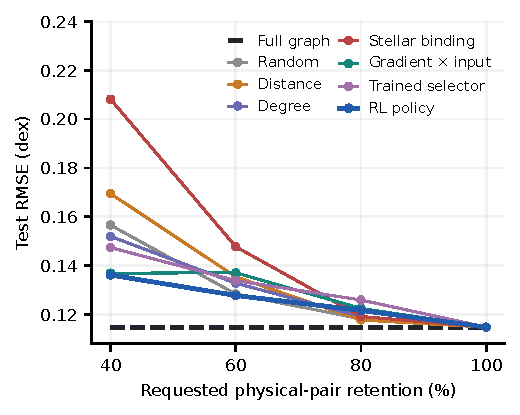
\includegraphics[width=\columnwidth]{figures/accuracy_tradeoff.pdf}
\caption{Accuracy across requested pair budgets (C). The full graph is a reference, not a sparsified mask at each abscissa. Lines join measured configurations; no unmeasured budgets or uncertainty bands are implied.}
\label{fig:tradeoff}
\end{figure}

Table~\ref{tab:accuracy} and Figure~\ref{fig:tradeoff} show convergence toward full-graph performance as retention increases. Full-graph RMSE is $0.114797\dex$. RL at 40\% gives $0.136160\dex$, an 18.61\% increase in error. Its MAE is $0.109011\dex$ and $R^2=0.874075$, compared with $0.090928\dex$ and 0.910491 for the full graph. Removing roughly 60\% of physical pairs therefore has a measurable accuracy cost for this predictor.

The strongest point-estimate sparse selector changes with budget. RL gives $0.127760\dex$ at 60\%, slightly below random's $0.128369\dex$ (a 0.47\% relative difference). At 80\%, distance gives $0.117740\dex$, below RL's $0.121663\dex$. At 100\% every selector recovers the full-graph result within floating-point noise. This is a useful consistency check on decoding and evaluation, but does not demonstrate that a selector generalizes. Gradient saliency is slightly non-monotone between 40\% and 60\%; more retained pairs need not monotonically improve each method's error under a frozen nonlinear predictor.

\subsection{Comparison with alternative selectors}
\label{sec:comparisons}
At 40\%, gradient~$\times$~input is the closest point-estimate competitor: $0.136900\dex$, versus RL's $0.136160\dex$. RL's relative RMSE advantage is approximately 0.54\%, and its MAE is slightly worse ($0.109011$ versus $0.108918\dex$). Thus even the aggregate metric chosen for ranking affects the descriptive conclusion. The trained selector gives $0.147382\dex$ and random gives $0.156571\dex$.

\begin{table*}[t]
\centering\small
\caption{Exploratory paired comparisons at $q=0.4$. $\Delta=\RMSE_{\mathrm{RL}}-\RMSE_{\mathrm{control}}$; negative favors RL. Intervals use 50,000 paired BCa draws. Two-sided permutation tests swap squared errors within halos (99,999 draws). Holm values adjust seven comparisons; intervals remain unadjusted.}
\label{tab:paired}
\begin{tabular}{lrrrr}
\toprule
Control & $\Delta$ (dex) & Marginal 95\% BCa interval (dex) & Paired $p$ & Holm $p$ (7) \\
\midrule
Gradient $\times$ input & -0.000739 & [-0.014508, +0.013582] & 0.91920 & 0.91920 \\
Random & -0.020411 & [-0.050979, +0.003193] & 0.18190 & 0.54570 \\
Trained selector & -0.011222 & [-0.022461, -0.001826] & 0.03774 & 0.15096 \\
Degree & -0.015781 & [-0.043872, +0.006982] & 0.26796 & 0.54570 \\
Distance & -0.033309 & [-0.057936, -0.008931] & 0.01550 & 0.07750 \\
Stellar binding & -0.071968 & [-0.095711, -0.044928] & 0.00004 & 0.00028 \\
Full graph & +0.021364 & [+0.011135, +0.032705] & 0.00022 & 0.00132 \\
\bottomrule
\end{tabular}

\end{table*}

\begin{figure}[t]
\centering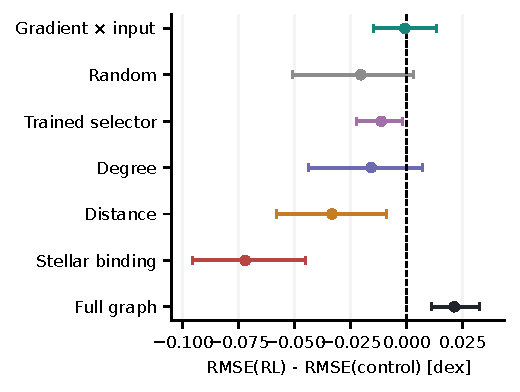
\includegraphics[width=\columnwidth]{figures/paired_uncertainty.pdf}
\caption{Paired RMSE contrasts and marginal 95\% BCa intervals at 40\% retention. Zero denotes equal RMSE. Intervals reflect halo-sample variation conditional on this policy, backbone, catalog, and split.}
\label{fig:paired}
\end{figure}

The paired RL--saliency RMSE difference is $-0.000739\dex$ with 95\% BCa interval $[-0.014508,+0.013582]\dex$ and permutation $p=0.9192$ (Table~\ref{tab:paired}; Figure~\ref{fig:paired}). The interval admits both benefit and harm. RL improves absolute error on 42 of 82 halos and worsens it on 40. A leave-one-halo-out analysis can reverse the sign of the RMSE gap. The observed difference is therefore unsuitable as evidence of a reliable advantage.

Against the single random test realization, the point difference is $-0.020411\dex$ (13.04\% relative improvement), but its interval $[-0.050979,+0.003193]\dex$ crosses zero and $p=0.1819$. Nominal contrasts with the trained selector and distance do not survive the seven-comparison Holm adjustment. The weak stellar-binding heuristic is clearly worse in this conditional analysis; beating it does not establish superiority over competitive selectors. The full graph is more accurate, with RL--full difference $+0.021364\dex$ and interval $[+0.011135,+0.032705]\dex$. Adjusting all 21 sparse-budget contrasts leaves the RL--full and RL--binding conclusions at 40\% below 0.05, while weakening other comparisons. These statements remain conditional on the sampling assumptions in Section~\ref{sec:stats}.

\subsection{Test-time adaptation}
\label{sec:tta}
D preserves exactly the same final pair counts across $K$ for each test halo. Its nominal 50\% budget realizes 51.01\% mean physical retention. The CSV's 56.25\% stored retention includes loops and must not be interpreted as the physical-pair fraction. All 82 test graphs pass the final budget and coverage checks.

\begin{table*}[t]
\centering\small
\caption{D adaptation at a separate requested 50\% pair budget. RMSE is in dex. $K$ is a maximum; early stopping reduces actual steps. $K=20$ was selected using validation only. Nine decimals expose the near-tie between $K=10$ and 20 and are not a claim of measurement precision.}
\label{tab:tta}
\begin{tabular}{rrrrr}
\toprule
$K$ & Validation RMSE & Test RMSE & s/halo & Steps \\
\midrule
0 & 0.127539232 & 0.131123230 & 0.468 & 0.00 \\
5 & 0.127231658 & 0.130803317 & 1.035 & 4.76 \\
10 & 0.127205506 & 0.130391479 & 1.166 & 6.15 \\
20 & 0.127205476 & 0.130391493 & 1.169 & 6.20 \\
\bottomrule
\end{tabular}

\end{table*}

Validation selects $K=20$; $K=10$ and 20 have essentially identical validation and test scores (Table~\ref{tab:tta}). Relative to $K=0$, selected adaptation lowers test RMSE from 0.131123230 to $0.130391493\dex$, an absolute change of $-0.000731736\dex$ and relative change of 0.558\%. MAE changes from 0.102724284 to $0.102651902\dex$, and $R^2$ from 0.883220 to 0.884520. Early stopping yields 6.20 mean steps at $K=20$. The original validation choice is retained despite the negligible difference from $K=10$; test scores do not determine the choice.

D exports aggregates, counts, and adaptation histories but no final per-halo predictions or residuals. Consequently no paired significance assessment of its small accuracy change is supported. Reducing dropout variability is also not guaranteed to reduce prediction error. These observations are descriptive evidence for the implemented adaptation procedure, not evidence of statistically established improvement or cross-domain robustness.

\subsection{Computational efficiency}
\label{sec:efficiency}
At 40\% retention C's RL inference region averages 0.44026 seconds per halo, versus 0.007839 seconds for the full reference: a $56.16\times$ slowdown. Mean scoring, decoder, and pruned-prediction times are approximately 0.01182, 0.41823, and 0.00844 seconds, respectively; the remaining difference is region overhead. CPU feasibility checks dominate the decoder. The measured pruned forward itself is not faster than the full reference in these small-graph runs. RL slowdowns rise to approximately $71\times$, $78\times$, and $83\times$ at 60, 80, and 100\% retention.

\begin{figure*}[t]
\centering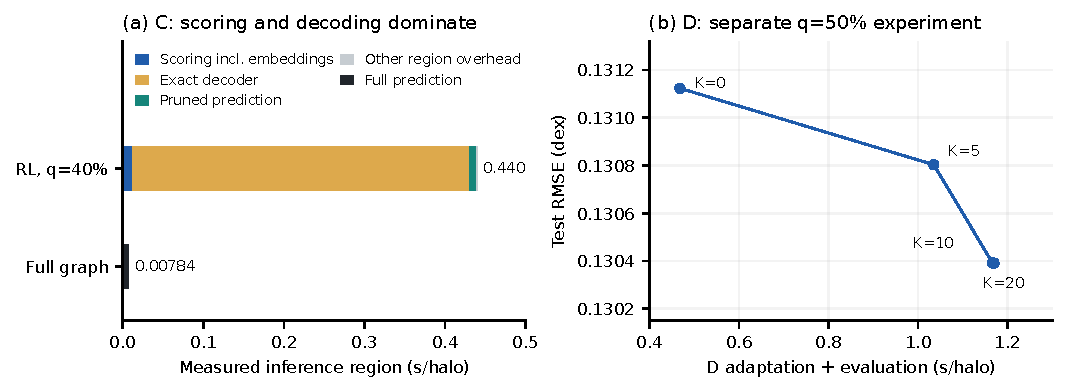
\includegraphics[width=0.96\textwidth]{figures/efficiency_and_tta.pdf}
\caption{Measured computational cost. (a) C's 40\% RL path includes live full-graph embeddings, policy scoring, exact decoding, and retained prediction. (b) D's label-free adaptation at a separate 50\% budget gives a small aggregate RMSE change with higher latency. Timing scopes differ between panels; these are observed campaign measurements, without repeated hardware benchmarking or timing confidence intervals.}
\label{fig:cost}
\end{figure*}

The scorer requires a full-backbone embedding pass before a second, sparse prediction pass. Per-halo records confirm two live predictor forwards for RL versus one for the full reference. Faster decoding alone therefore would not demonstrate an end-to-end speedup over this same backbone. Computation reuse or a cheaper encoder would require a different implemented path and fresh measurements. Graph construction takes 0.8518 seconds for the built split set and is reported separately; recovered historical RL training cost is unknown, not zero.

For D, $K=0$ costs 0.468 seconds per halo and $K=20$ costs 1.169 seconds, a $2.498\times$ latency increase (Figure~\ref{fig:cost}). This cost accompanies a 0.558\% aggregate RMSE reduction without paired uncertainty. No measured amortized speedup, memory reduction, or accuracy--latency deployment advantage is established by these experiments.

\subsection{Additional diagnostics and fine-tuning}
Pair-collapsed physical-alignment analysis gives mean within-halo Spearman correlation 0.376 and median 0.410 between policy keep scores and the stellar binding proxy, with 78/82 positive correlations. This describes association, not causal physical relevance; edges share nodes and the proxy omits most halo matter. No reward or constraint ablation identifies which component causes the predictions.

Thirty-draw dropout intervals constructed as mean $\pm1.96$ standard deviations cover all 82 targets, with mean widths of 1.9596 dex for the full graph and 1.9499 dex for RL. Such broad uncalibrated intervals do not establish useful 95\% calibration or sharp uncertainty. These intervals concern dropout predictions and are distinct from the paired bootstrap intervals above.

B's optional supervised fine-tuning accepts epoch 2 after six executed epochs, because validation pruned RMSE improves from 0.123302 to 0.122764 dex and full-graph validation error remains within the 2\% tolerance. Test accuracy worsens: full RMSE increases from 0.114797 to 0.118644 dex, and pruned RMSE from 0.136160 to 0.137266 dex. One topology-infeasible training graph is excluded from this optional stage (377/378 eligible), without enlarging budgets; the original policy training population remains 378. The negative generalization result is retained, and C's primary comparisons use the unchanged frozen backbone.

\section{Discussion}
The strongest supported contribution is a traceable benchmark for constrained selection. Reciprocal copies and architecture loops can conceal budget mismatches if all stored columns are treated as independent actions. Counting physical pairs, recording final masks, checking feasibility before evaluation, and using one decoder make the comparison interpretable. These checks matter even when the learned method does not improve the downstream objective.

Three failure modes are visible. First, a repaired sampling environment and a constrained inference environment can expose a policy to different mask distributions. Exact inference guarantees the declared graph contract but does not retroactively change the objective used to fit the policy. Second, the relative virial term preserves a tracer-based reference that may itself be systematically displaced from a true halo equilibrium quantity. Its usefulness for accuracy requires an ablation rather than an appeal to the virial theorem. Third, small-graph savings can be overwhelmed by matching-based feasibility checks and the full embedding pass. Counting removed edges alone would miss this computational disadvantage.

The small RL--saliency gap illustrates why matched budgets must be accompanied by paired uncertainty and competitive controls. Selecting the largest apparent gain over a weaker heuristic would hide the central ambiguity. Similarly, a validation execution gate is a selection rule, not evidence of test significance. The optional backbone fine-tuning and adaptation results show that internally acceptable updates can give weak or unfavorable changes in held-out accuracy. Deployment requires a useful effect at a justified cost, not merely a successful optimization run.

\section{Limitations}
\label{sec:limitations}
\paragraph{Historical semantics and provenance.}
The CSV's historical mass definition is unresolved, and its radius is total-subhalo rather than certified stellar type-4 radius. Input hashes and frozen-state checks do not certify the original HDF5 field mappings, acquisition filters, metallicity definition, periodic treatment, or backbone training/test separation. The checkpoint architecture can be inspected without reconstructing its full training provenance. Absolute astrophysical performance claims remain conditional on those unresolved issues.

\paragraph{Replication and domains.}
The halo split samples one simulation volume. There is one fitted policy, no independent policy-seed replication, and one random test realization. Halo-bootstrap intervals omit policy, backbone, and volume variation and may understate uncertainty under spatial dependence. No completed CAMELS, SIMBA, observational-noise, or independent-volume validation supports transfer claims. The small observed graphs limit claims about larger systems.

\paragraph{Objective, inference, and uncertainty.}
There are no completed physics-reward, constraint, feature, or repair ablations, and no certified observational input experiment. The raw selector is one modest trained control rather than a tuned state-of-the-art baseline. TTA lacks exported paired predictions; dropout-uncertainty reduction can occur without accuracy improvement. Calibration, conditional coverage, peak memory, repeated timing variation, and total training amortization remain unmeasured. The benchmark is controlled within its stated contract, but not an exhaustive comparison of selectors.

\paragraph{Proposed work, not completed findings.}
A confirmatory study should first certify target and feature semantics and train a fresh compatible backbone with complete split and augmentation records. It should reserve independent initial conditions or volumes for confirmation; predeclare the retention budget, primary comparator, and meaningful effect or non-inferiority margin; and replicate policy/backbone seeds and random test masks. Further experiments should ablate physical terms and constraints, export TTA predictions and masks, and measure repeated end-to-end cost on larger graphs. The repository's separate audited projected-data path does not yet supply a validated compatible policy reward/trainer; missing intrinsic features must not be zero-filled to reuse this policy. These are future experiments and implementation requirements, not results of A--D.

\section{Conclusion}
Cosmic-Net's completed campaign demonstrates exact physical-pair budget enforcement and reproducible matched-population evaluation of a recovered RL selector. On 82 legacy-catalog test halos, nominal 40\% RL selection is 18.61\% worse in RMSE than the full graph, while its 0.54\% observed advantage over gradient~$\times$~input is unresolved by paired analysis. The implemented RL path is approximately $56\times$ slower. Label-free adaptation at a separate 50\% budget produces a 0.558\% aggregate RMSE reduction at $2.50\times$ latency, with insufficient exports for a paired test. The evidence supports an engineering and empirical analysis of constrained graph selection, with no established accuracy or efficiency advantage. Certified provenance, independent replications, and redesigned cost accounting are necessary before stronger scientific or deployment claims.

\paragraph{Availability and review status.}
This supervisor-review draft accompanies the source, BibTeX database, generated figures and tables, evidence snapshots with SHA-256 identities, a claim--evidence matrix, and an explicit missing-evidence register. Author affiliations, funding, and any formal data-release arrangements require confirmation before submission. The layout is a conventional two-column article and makes no claim of compliance with a particular venue template.

\label{page:main-end}
\clearpage
\bibliographystyle{unsrtnat}
\bibliography{references}
\clearpage
\onecolumn
\appendix
\section{Implementation and Artifact Traceability}
The accompanying \code{evidence/claim-evidence-matrix.md} maps empirical claims to exact source artifacts, row filters, and derivations. \code{evidence/source-manifest.json} records original absolute paths, campaign-relative paths, uncompressed SHA-256 hashes, and committed snapshot hashes. Large JSON files are losslessly gzip-compressed. Compressed snapshots can be verified and read without the original checkout. The manuscript asset script recomputes aggregate RMSE from C's saved predictions and verifies exact pair membership, loop retention, and physical coverage from serialized masks.

The campaign sessions are A: 358697902; B: 358708561; C: 358713276; D: 358778452. They are completed private Kaggle executions. Source commit \code{c825bf57652005c80faff79cf4dfd58e3a9baa14} governs the evaluated pipeline. The recovered policy's training source is \code{aeb5dad65d681728d525fb78a4ab919b0432ab90}; its relevant pair-training, policy, and reward modules agree with the campaign base. The new manuscript does not rerun training or replace any campaign artifact.

The input CSV SHA-256 begins \code{6c148f2cae68abac}, and the frozen checkpoint file begins \code{42764f0db204863b}. The frozen parameter-state hash begins \code{56907374794d9203}; the file hash and state hash describe different objects. The recovered selected policy file hash begins \code{b1f41771c102bec6}. Full hashes and identities are retained in the evidence files. None of these hashes certifies the historical scientific semantics of the file contents.

\begin{table}[H]
\centering\small
\caption{Code paths defining the reported method at the campaign base. Function names identify the implementation, not a claim that every alternate repository path was executed.}
\label{tab:code}
\begin{tabular}{>{\raggedright\arraybackslash}p{0.26\textwidth}>{\raggedright\arraybackslash}p{0.38\textwidth}>{\raggedright\arraybackslash}p{0.27\textwidth}}
\toprule
Component & File and entry point & Role \\
\midrule
Node/target conversion & \code{data/loaders/base\_loader.py}: \code{SubhaloData.get\_node\_features}, \code{HaloData.log\_halo\_mass} & Four logs and stored target \\
Graph geometry & \code{graph/graph\_builder.py}: \code{\_build\_standard\_graph}, \code{\_compute\_edge\_features} & Radius graph, loops, fallback, attributes \\
Predictor & \code{model/model.py}: \code{CosmicNetGNN}, \code{NNConvBlock} & Frozen edge-conditioned GNN \\
Pair training & \code{rls/pair\_training.py}: \code{train\_pair\_policy}; \code{rls/pair\_policy.py}: \code{pair\_mask} & Ordered actions, repair, rollout baseline \\
Physical reward & \code{rls/train\_policy.py}: \code{\_graph\_physics\_terms}; \code{rls/rewards.py} & Loop-free reference-relative proxy \\
Exact feasibility & \code{rls/constraints.py}: \code{minimum\_additions}; \code{rls/constrained\_policy.py}: \code{select\_pairs} & Matching-based completion and ranking \\
Scorers and benchmark & \code{rls/benchmark\_scorers.py}; \code{rls/matched\_benchmark.py} & Common budgets and cost accounting \\
Adaptation & \code{rls/pair\_tta.py}: \code{adapt\_pair\_policy} & Label-free rollouts and exact final mask \\
\bottomrule
\end{tabular}
\end{table}

\section{Recorded Settings and Recovery Limits}
\begin{table}[H]
\centering\small
\caption{Recorded campaign and policy settings. Backbone settings specify the loaded architecture; they are not a certified historical backbone training recipe.}
\begin{tabular}{llll}
\toprule
Setting & Value & Setting & Value \\
\midrule
Node / edge dimensions & 4 / 5 & GNN layers / width / output & 3 / 64 / 64 \\
Pooling / dropout & mean / 0.05 & Radius / self-loops & 2.0 Mpc / retained \\
Policy width / normalization & 64 / train-fitted & Epochs / selected epoch & 60 / 42 (zero-based) \\
Policy Adam rate / batch & $10^{-3}$ / 32 graphs & Rollouts / gradient clip & 4 / 1.0 \\
Keep curriculum & 0.9 to 0.4 in 40 epochs & Entropy / value weights & 0.01 / 0.5 \\
Reward error scale (recovered) & 0.124135822 dex & Constraint / decoder & no isolates / direct \\
TTA Adam rate / MC draws & $10^{-4}$ / 15 & TTA patience / keep & 3 / 0.5 \\
TTA KL / rate decay & 0 / 1 & Random validation seeds & 10 \\
\bottomrule
\end{tabular}
\end{table}

The recovered training metadata explicitly marks the reward scale as reconstructed from the exact training inputs and frozen predictions. Its CPU float32 reconstruction is not asserted to be bitwise identical to the original GPU scalar. Normalization buffers are compatible with the recovered data and the replayed validation RMSE differs by approximately $6\times10^{-8}$ dex. Original policy weights and logs are retained. Missing optimizer and RNG states mean recovery supports inference evaluation, not exact resumption of an interrupted optimizer trajectory.

One optional Stage B training graph, \code{tng100\_0000005}, has $P=12$ pairs, requested $\lceil0.4P\rceil=5$, but minimum no-isolate edge cover 6. The exact decoder correctly rejects that request. A topology-only eligibility report excludes it from optional backbone fine-tuning; all 81 validation and 82 test graphs remain eligible. Exclusion was not based on its residual, and no budget was increased. This case illustrates why a minimum-fraction threshold is insufficient to guarantee feasibility.

\section{Per-Halo Diagnostics}
\begin{figure}[H]
\centering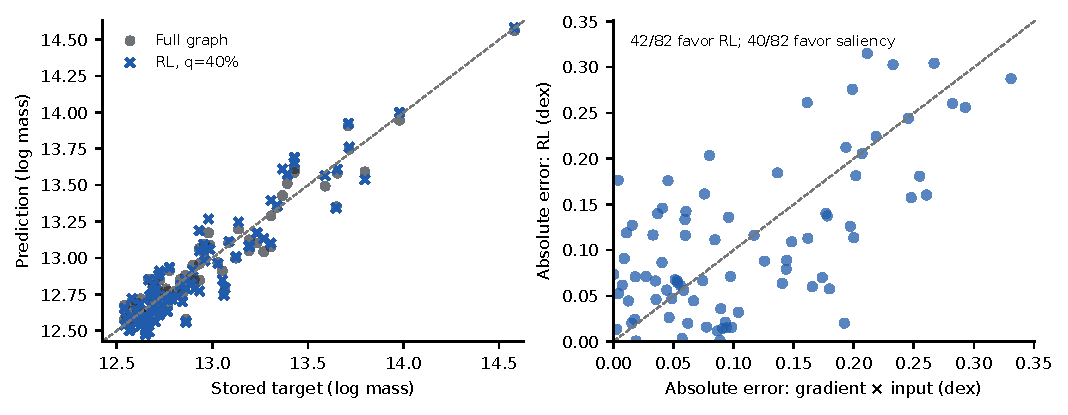
\includegraphics[width=0.96\textwidth]{figures/per_halo_diagnostics.pdf}
\caption{C's saved per-halo predictions at requested 40\% retention. Left: full and RL predictions versus the stored logarithmic target. Right: RL and gradient~$\times$~input absolute errors on identical halos; points below the diagonal favor RL. These plots expose heterogeneity within the aggregate near-tie, without adding independent experimental units.}
\label{fig:halos}
\end{figure}
Figure~\ref{fig:halos} uses the same 82 halos as the main tables. Multiple methods and budgets do not enlarge this sample. The paired statistical export also records leave-one-halo-out RMSE contrasts and Holm-adjusted results for all 21 nontrivial-budget contrasts. These diagnostics support sensitivity assessment, not independent confirmation after test-set inspection.

\section{Missing Evidence and Proposed Confirmation}
No fabricated result panels are supplied for unavailable experiments. The following gaps are explicit placeholders for future evidence: certified catalog field/target semantics and original checkpoint training provenance; independent policy/backbone seeds and volumes; actual cross-simulation and observational validation; physical-reward, feature, and constraint ablations; per-halo final TTA predictions and masks; calibrated uncertainty and repeated hardware/memory measurements. The machine-readable campaign exports do not provide those results. The companion \code{evidence/missing-results.md} prioritizes them and specifies what would resolve each gap.

The current evidence can support supervisor discussion of feasibility, methodology, effect sizes, and computational failure modes. It is insufficient to declare a new astrophysical mass calibration, robust RL superiority, or deployment efficiency. A later confirmatory study must use new independent evidence and report changes to dataset, objective, checkpoint, and selection protocol explicitly.

\end{document}
